%% journal.tex
%% V1
%% 20014/03/06
%% by Maarten Hattink

\documentclass[10pt,conference]{IEEEtran}

\IEEEoverridecommandlockouts
% Used space can be reduced by tweaking line 4478 of the .cls template file :)
%\IEEEpubid{\makebox[\columnwidth]{\hfill 978-3-9815370-0-0/DATE13/\copyright2014 EDAA} \hspace{\columnsep}\makebox[\columnwidth]{ }}

% *** GRAPHICS RELATED PACKAGES ***
%
\ifCLASSINFOpdf
  \usepackage[pdftex]{graphicx}
  % declare the path(s) where your graphic files are
  \graphicspath{{img/}}
  % and their extensions so you won't have to specify these with
  % every instance of \includegraphics
  \DeclareGraphicsExtensions{.pdf,.jpeg,.png}
\else
  % or other class option (dvipsone, dvipdf, if not using dvips). graphicx
  % will default to the driver specified in the system graphics.cfg if no
  % driver is specified.
  \usepackage[dvips]{graphicx}
  % declare the path(s) where your graphic files are
  \graphicspath{{img/}}
  % and their extensions so you won't have to specify these with
  % every instance of \includegraphics
  \DeclareGraphicsExtensions{.eps}
\fi

\usepackage[cmex10]{amsmath}
\usepackage{array}
\usepackage{paralist}
\usepackage{cite}
\usepackage[T1]{fontenc}
\usepackage{fancyhdr}
\usepackage{color}
\usepackage{acronym} % Automated abbreviations
\usepackage[table]{xcolor}
\usepackage{url}
\usepackage{tabularx}

\pdfinfo{
   /Author (Maarten Hattink)
   /Title  (Bringing stereo sound to real-time CompSOC platform)
   /Subject (Bringing stereo sound to real-time CompSOC platform)
   /Keywords (Virtual, Composable, CompSOC)
}

\definecolor{gray}{rgb}{0.5,0.5,0.5}
\definecolor{grayl}{rgb}{0.8,0.8,0.8}

% Abbreviations:
\acrodef{SoCs}[SoCs]{Systems-on-Chips}

% Old-style abbreviations and commands
\newcommand{\pmodfull}{PmodI\textsuperscript{2}S }
\newcommand{\digipmod}{Digilent \pmodfull }
\newcommand{\cirruslogic}{Cirrus Logic CS4344 Stereo D/A converter}
\newcommand{\cs}{CS4344}

% Utilities:
\newcommand{\bulletversion}[1]{{\color{black} #1}}
\newcommand{\oldbulletversion}[1]{{\color{gray} #1}}
\newcommand{\redcomment}[1]{{\color{red} \emph{#1}}}
\newcommand{\citn}[1]{{\color{blue} \emph{$^\text{citation needed}$}}}
\newcommand{\todo}[1]{{\color{blue} \emph{TODO: #1}}}
\newcommand{\bluecomment}[1]{{\color{blue} \emph{#1}}}
\newcommand{\graycomment}[1]{{\color{gray} \emph{#1}}}
\newcommand{\hide}[1]{}

% correct bad hyphenation here
\hyphenation{op-tical net-works semi-conduc-tor}

% Note: -2em vspace applied to figures + table
\renewcommand{\baselinestretch}{0.95}
\newcommand{\reducespace}{{\vspace{-1.7em}}}
\newcommand{\reducefigtocapspace}{{\vspace{-0.2em}}}
\newcommand{\reducetablespace}{{\vspace{-2em}}}
\newcommand{\reducecaptotablespace}{{\vspace{-0.5em}}}

\begin{document}
%
% paper title
% can use linebreaks \\ within to get better formatting as desired
\title{Bringing Stereo Sound to the FPGA Based \\CompSOC Platform}

% author names and affiliations
% use a multiple column layout for up to three different
% affiliations
\author{\IEEEauthorblockN{Maarten Hattink}
\IEEEauthorblockA{Eindhoven University of Technology, Eindhoven, The Netherlands}}

% make the title area
\maketitle

%%%%%%%%%%%%%%%%%%%%%%%%%%%%%%%%%%%%%%%%%%%%%%%%%%%%%%%%%%%%%%%%%%%%%%%%%%%%%%%%%%%%%%%%%%%%%%%%%%%%%%%%%%%%%%%%%%%%%%%%%%%%%%%%%%%%
%%%%%%	ABSTRACT
%%%%%%%%%%%%%%%%%%%%%%%%%%%%%%%%%%%%%%%%%%%%%%%%%%%%%%%%%%%%%%%%%%%%%%%%%%%%%%%%%%%%%%%%%%%%%%%%%%%%%%%%%%%%%%%%%%%%%%%%%%%%%%%%%%%%
\begin{abstract}
In the modern Connected World systems are highly integrated and execute many applications. The CompSOC platform is designed to make independent development and verification of those applications possible. Those applications also need to communicate with the rest of the world. A method of doing this is by using sound. This paper discusses a sound module for the CompSOC platform. This module is designed to connect a \digipmod to the platform to enable the use of audio signals by applications executed on it. The module consists of hardware implemented in the CompSOC's FPGA and an API which can be used by programmers to use it. The sound module is highly flexible and can be configured by the applications using it at run time. The module's design and implementation are explained in-depth as well as the verification process used.
\end{abstract}

\IEEEpeerreviewmaketitle

\IEEEpubidadjcol

%%%%%%%%%%%%%%%%%%%%%%%%%%%%%%%%%%%%%%%%%%%%%%%%%%%%%%%%%%%%%%%%%%%%%%%%%%%%%%%%%%%%%%%%%%%%%%%%%%%%%%%%%%%%%%%%%%%%%%%%%%%%%%%%%%%%
%%%%%%	INTRODUCTION
%%%%%%%%%%%%%%%%%%%%%%%%%%%%%%%%%%%%%%%%%%%%%%%%%%%%%%%%%%%%%%%%%%%%%%%%%%%%%%%%%%%%%%%%%%%%%%%%%%%%%%%%%%%%%%%%%%%%%%%%%%%%%%%%%%%%

\section{Introduction}
In our modern day society everything becomes connected to everything, creating a Connected World. This causes many applications to be integrated in single systems. Often, those applications are developed independently before being integrated. This integration proves to be very difficult and may pose many problems. One of those problems are timing issues that arise when running multiple applications on one processor. Applications that previously executed perfectly, may not meet their requirements when other processes use shared resources. To solve these problems, the Composable System On a Chip (CompSOC) platform has been developed. Its design is explained in-depth in~\cite{goossens2013virtual}.

The applications executed on CompSOC have to communicate with their human users. One form of this communication is through sound. This paper describes a hardware module, implemented in the CompSOC's FPGA, that allows applications to use a \digipmod~\cite{pmodsheet}  to produce stereo channel audio signals. The audio's sample rate is configurable and its range includes the 48 kHz frequency recommended in~\cite{aesrecommendation}. Also a thin software layer, the Application Programming Interface (API),  has been developed to allow for easy interfacing with the hardware module by applications that execute on CompSOC. The goal for this API is to be flexible and easy to use. Another important part of the project was the verification of the module's functionality, which is done through simulations and signal measurements. 

This paper first provides background information on the CompSOC platform in Section~\ref{sec:background}. Following, the hardware module's design and considerations are discussed in Section~\ref{sec:hardware}. Then, in Section~\ref{sec:software}, the API is described shortly. After that Section~\ref{sec:verify} shows the verification process and its results. Finally, some concluding remarks are made in Section~\ref{sec:conc}.

%%%%%%%%%%%%%%%%%%%%%%%%%%%%%%%%%%%%%%%%%%%%%%%%%%%%%%%%%%%%%%%%%%%%%%%%%%%%%%%%%%%%%%%%%%%%%%%%%%%%%%%%%%%%%%%%%%%%%%%%%%%%%%%%%%%%
%%%%%%	BACKGROUND
%%%%%%%%%%%%%%%%%%%%%%%%%%%%%%%%%%%%%%%%%%%%%%%%%%%%%%%%%%%%%%%%%%%%%%%%%%%%%%%%%%%%%%%%%%%%%%%%%%%%%%%%%%%%%%%%%%%%%%%%%%%%%%%%%%%%
\section{Background}\label{sec:background}
One of the many problems when integrating different applications, developed by different teams, is that they interfere with other applications in the system. During development, this interference does not exist. This makes the development environment different from the final product environment, which can cause problems like applications not meeting their timing constraints. The verification of these systems is therefore becoming a major problem, as the verification process has to be repeated every time an application is modified. Solving this problem requires a predictable and composable platform. Such a system allows for independent development, verification and execution of applications by eleminating interference between them. The CompSOC platform tries to meet these requirements using propositions in~\cite{akesson2009composable}. This results in a platform that offers the possibility to execute applications that always behave the same, regardless of any other application being executed at the same time, even when those application share the available resources.

CompSOC consists of multiple MicroBlaze soft processor cores,~\cite{microblaze}, a Network on a Chip (NoC) and several I/O blocks. One of the most important elements is the NoC, it has to provide guaranteed bandwidth and latency to dynamically started and halted processes. The principles on which it operates are described in~\cite{hansson2011chip}. Other I/O blocks, such as the sound module described in this paper, are connected to the NoC using a network interface and a simplified version of the DTL protocol. Even in its simplified form, the DTL protocol is quite complex to implement correctly. If not implemented properly, logic paths can become too long, causing the system to be forced to use a slower clock than otherwise possible. A slower clock would result in a severe performance penalty and must be avoided. Therefore a proxy is used, which handles the specific timings of signals and provides buffering of the DTL signals. Thereby it prevents the logic path from becoming longer than allowed, reducing the complexity of the sound module itself. The DTL protocol works with a master and a slave interface. The master interfaces are located in the CompSOC's processors and the slave interfaces in the I/O blocks. The interfaces consist of three groups of signals, the command, read and write groups. First a DTL command to the module is issued over the command signals. The command indicates if it is a read from or a write to the I/O block. It also contains the address where the read or write has to take place. All data is sent via 32 bit data connections in the read and write signal groups.

The purpose of the developed sound module is to control the \pmodfull module. The Pmod's main component is a \cirruslogic,~\cite{cirruslogic}. It converts 16 or 24 bit audio samples to an analog signal, which is output via the 1/8-inch stereo jack on the Pmod. The \cs~requires four signals from CompSOC to operate. These signals are the Master Clock (MCLK), the Left Right Clock (LRCK), the Serial Clock (SCLK) and the Serial Data Input (SDIN). The SDIN carries the audio data, which is serially clocked into the chip. The MCLK is the clock signal on which the \cs~operates and derives internal clock signals from. The LRCK  indicates to the \cs~for which audio channel the data on the SDIN is meant. A logic-low signal means the data is for the left audio channel, while a logic-high signal means it is meant for the right audio channel. The frequency of the LRCK is also equal to the sample rate of the audio signal. The SCLK is the clock signal for the data on the SDIN, which is sampled at the SCLK's rising edge. Using these four signals the \cs~can be configured and used to generate two audio signals, the left and right channels. The sample data the \cs~accepts are in 16 or 24 bit two's complement values.

%%%%%%%%%%%%%%%%%%%%%%%%%%%%%%%%%%%%%%%%%%%%%%%%%%%%%%%%%%%%%%%%%%%%%%%%%%%%%%%%%%%%%%%%%%%%%%%%%%%%%%%%%%%%%%%%%%%%%%%%%%%%%%%%%%%%
%%%%%%	HARDWARE
%%%%%%%%%%%%%%%%%%%%%%%%%%%%%%%%%%%%%%%%%%%%%%%%%%%%%%%%%%%%%%%%%%%%%%%%%%%%%%%%%%%%%%%%%%%%%%%%%%%%%%%%%%%%%%%%%%%%%%%%%%%%%%%%%%%%
\section{Hardware module}\label{sec:hardware}
\subsection{Design considerations}
A number of requirements have to be fullfilled by the hardware module's design. First, the three necessary clock signals have to be generated. All clock signals' frequencies depend on each other. The ratio between the MCLK's and LRCK's frequencies can only be chosen from a set of ten integer values, which can be found in~\cite{cirruslogic}. Also, SCLK's frequency needs to be at least $2N$ times higher thatn LRCK's frequency, where $N$ is the number of bits per sample. Second, the audio samples need to be provided to the Pmod continuously, even if the producing application is halted out by the operating system temporarily to execute another application. Third, the module has to be flexible. It has to be able to work at multiple sample rates, be able to produce two separate audio signals on the different channels or the same signal on both, and be composable. Applications also have to be able to configure the module at run time, to make multiple configurations during the application's lifetime possible. 

The first requirement is met by generating all clock signals from one clock in the module itself. It might also have been possible to use the FPGA's clock generators to produce the proper signals, but this option was discarded due to the limited availability of those resources. Also it was expected that in such implementation would be difficult to synchronize the clock signals. Therefore the clocks are generated hierarchically from high frequency to slow frequency. First the MCLK is generated from the system clock, then the SCLK from the master clock and finally the LRCK is generated from the SCLK. 

To keep producing audio signals when an application is not actively sending data requires a sample buffer. The design of the audio buffer determines many of the final system's capabilities. For example, a circular buffer allows for replaying old audio sample's, reducing the amount of required processing by the CompSOC's CPU. A circular buffer also costs a greater amount of the available resources on the FPGA compared to a simpler First In First Out buffer (FIFO), but a FIFO cannot reuse samples. Another consideration in designing the audio buffer is the dataformat in which samples are presented. Because the DTL interface provides with 32 bit data channel and it is assumed that the noiselevel of the \cs~is significant compared to the contribution of the last few bits, every data transmission via the DTL interface will contain two 16 bit samples, sacrificing precision for a larger transfer rate. First it was decided to implement the more flexible circular buffer, but an early prototype of the buffer showed that it costs a large amount of resources. Therefore a sacrifice on flexibility is made and a FIFO implementation, available from the CompSOC's library, used. The readily available and extensively tested FIFO also made time consuming verification of the buffer itself unnecessary. A final design aspect of the buffer is its size. A large buffer requires a lot of hardware, but a small buffer requires a lot of updates per second to keep it filled. Many updates per second increase overhead on the processor's side, so a balance between the update rate and buffer size has to be found. Fig.~\ref{fig:buffersize} shows the calculated minimum buffer size versus the minimum updates per second. A feasible estimate of the update rate is 50 updates per second. At a sample rate of 48 kHz that requires, with a small extra margin, a buffer of 1024 samples for each channel. Due to the dependency on the sample rate the module is designed such that the buffer size can be easily changed when synthesizing CompSOC for the FPGA. 
\begin{figure}[h]
 \includegraphics[width=0.5\textwidth]{buffersize}
 \caption{Graph showing the minimum buffer size in samples, per channel, versus the minimum required updates per second. Also the chosen 1024 samples, with the minimum of 50 updates per second is indicated at the intersection of the red lines .}
 \label{fig:buffersize}
\end{figure}

The final important design consideration is the composability of the sound module. Composability requires that the module can be shared between applications without letting them interfere with each other. Because the module has to keep producing audio signals when an application is not active, it cannot be timeshared between different applications. However, it may be divided into multiple resources. It can be designed in such manner that applications can request seperate access to one or more of the audio channels and the configuration of the sound module. If an application would only have access to one audio channel, it would be able to read the configuration of the signals from the module. This would still cause some interference between applications, but that cannot be changed by the design of the module without sacrificing its flexibility. For example, the both audio channels must have the same sample rate. If an application does not have control over the sample rate, it is influenced by the application that does. These problems can be countered by designing all applications that run on the system for the same audio settings, resulting in a module that is composable for independent design and verification. The downside of such an implementation is the resource requirement. Every seperate part of the module, that acts as a single resource to an application, requires its own connection to the NoC. The design of the NoC requires that for each connection to it a minimum amount of bandwidth is allocated to that connection. Audio data does not require that amount of bandwidth, resulting in reduced utilization. Moreover, in usecases where a single application uses the entire sound module the separate connections are not necessary, as a single connections has enough bandwidth for the entire module. To minimize costs the module will only have one DTL connection to the NoC and  can only be used by one application. From that application's viewpoint the module will, however, be composable. The configuration of the module at run time is made possible by configuration registers inside the hardware module. Those registers are written to with special commands that are sent via the same DTL connection as the sound data.

\subsection{Implementation}
A global overview of the sound module's hardware final implementation is shown in Fig.~\ref{fig:overview}. The module consists of the DTL proxy, a controller that sends data to the correct submodules, two sample buffers, the clock generators and the output controller. The DTL proxy converts the NoC's DTL protocol to a simplified version, reducing the complexity of the data flow controller and preventing problems with signal timing and logic path length. Data coming in over the NoC is sent to either the sample buffers or stored in registers in the data flow controller. Settings can also be read from the module, which is also handled by the dataflow controller. The audio buffers are implemented as FIFO buffers. The clocks are generated and synched in the clock generator module, which itself consist of two identical generators that derive a slower clock from a faster clock. Those two generators create the SCLK and LRCK signals and the MCLK is generated by a different module based on the system clock. Finally the output controller controls the SDIN signal using the configured settings, samples and clock signals. More detailed descriptions of the submodules are given below. They explain how the modules are implemented and where necessary why that implementation is chosen. Also the effects of the implementation are discussed.
\begin{figure}[h]
 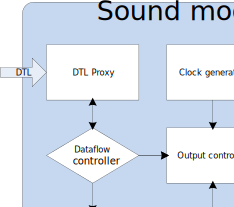
\includegraphics[width=0.5\textwidth]{PmodModuleOverview}
 \caption{The global structure of the sound module}
 \label{fig:overview}
\end{figure}
\subsubsection{Dataflow controller}
The dataflow controller is implemented as a Finite State Machine (FSM) with five states. First it will process the command signals on the DTL interface in its base command state. If the command is a read it will continue to its read state, but in case of a write the next state depends also on the commands address. The command's address indicate whether it is a write to the audio buffers or to configuration registers. Both options have a corresponding state. The fifth state is for burst writes to the registers, which do not have any effect. However, the fifth state is necessary to properly receive and drop those writes if they occur. 

\subsubsection{Audio buffers}
For the audio buffer an implementation with shift registers is chosen. This required the least resources of the four implementations available in the CompSOC's library. Buffer over- and underflows are handles as follows. Overflows cause the module to stop accepting new samples and the underflows force insertion of empty samples in the audio stream. Using this property of the FIFO it is possible to disable a single audio channel by not sending samples to it. The zeroes are inserted into the stream and the \cs~will set the output to zero, effectively disabling the channel. 

\subsubsection{Clock generators}
The three clock signals are derived from each other and effectively all based on the system clock. First the MCLK is generated by a clock divider that can be configured through the sound module's registers. This divider can divide the system clock by any positive integer that can be stored in seven bits. But only dividing by one, or a multiple of two results in a stable 50 percent duty cycle MCLK. Both the SCLK and LRCK are produced by instances of the same clock divider. This divider can also only create stable 50 percent duty cycle clocks if it divides by one or a multiple of two, but has a smaller range of possible division values. This range is configureable when synthesizing the sound module. The reason for not using this generator to generate the MCLK is that it uses the system clock as a clock for the counter registers and the input base clock as an enable signal for those registers. If system clock would be used as the enable signal this would result in unpredictable behaviour which is unacceptable. The sound module can be modified to use a different base clock which, if that base clock is sufficiently slower than the system clock, can be used as an enable signal, allowing for the reuse of this clock divider. Another effect of using the base clock as an enable signal is some jitter on the resulting clock signal, but this has proven to be acceptable for the \cs. The SCLK is based on the MCLK. The ratio between the two clocks is configurable and depends on the ratio between the MCLK and LRCK. In turn the LRCK is based on the SCLK with a fixed ratio of 64. This results in 32 SCLK periods per sample, enough to transfer a 24 bit sample, while using a suitable division ratio. After being phase synched with some extra registers, the clock signals are passed to the output controller that will either enable or disable them depending on the system's state. This synchronization is necessary to obtain the waveforms shown in Fig.~\ref{fig:clocks}, which is taken from~\ref{cirruslogic}. Notable characteristics are the falling edges of SCLK and LRCK, which take place at the exact same moment. Also the extra period of SCLK before sampling the Most Significant Bit (MSB) of the audio sample is an important requirement of \cs. The final important characteristic is that having more SCLK periods than bits in the sample has no effect. But to make sure the sample is not changed, the sound module holds SDIN at logic-low after the last bit.
\begin{figure*}[t]
 \includegraphics[width=\textwidth]{clocks}
 \caption{A representation of the LRCK, SCLK and SDIN signals. It shows the required phase synchronization the signals and sampling moments of SDIN.}
 \label{fig:clocks}
\end{figure*}

\subsubsection{Output controller}
The output controller handles events like activation and deactivation of the sound module. It also sets SDIN based on the SCLK, LRCK and the availability of samples. The activation sequence of the Pmod is relatively easy and starts with activating MCLK for 250 miliseconds before activating LRCK and SCLK. To complete the sequence, and enter the external SCLK mode of the \cs, the LRCK and SCLK have to be active for 16 periods of LRCK while SDIN is on a logic-low level. This is implemented by a FSM with a five states which are off, initialization step one, initalization step two, on, and deactivation one. In the first state all output signals are on a logic-low level. In the second state only MCLK is active and in the third also LRCK and SCLK are activated. In the fourth state the system is active and audio samples are sent to the Pmod. Finally, in the fifth state all signals are disabled for 250 miliseconds to discharge a capacitor on the Pmod. The final step prevents any glitches in the system if it is shutdown and started in quick succession. The control of SDIN is done by setting the next bit of a sample on the falling edges of SCLK so they are correctly sampled on SCLK's rising edge. As the samples are 16 bits long and 32 periods of SCLK pass during a half LRCK period, SDIN is set to logic-low when all 16 bits are transferred and transmission restarts on the next sample. Another feature implemented by the output controller is the mirroring of the left audio channel. This copies the samples from the left channel buffer to the right channel output. Doing so allows applications to only sent data to the left channel and still have it played on both channels, reducing the required processing power and communication.

\subsubsection{Hardware costs}
The hardware cost of the module is calculated as the fraction of used register and lookup table slices. The hardware usage of the sound module and reduced CompSOC are shown in Table~\ref{table:hardware}. It shows the number of available slices, the number used by CompSOC, and by the sound module. It also shows the fraction of used hardware by CompSOC and what part of CompSOC's hardware is used for the sound module. Most of the used LUTs are part of the audio buffers, whose size can be changed easily. Therefore the number of LUTs used can be changed if necessary. Another important value in cost calculation is the maximum allowed frequency of the system clock. For the reduced CompSOC with sound module the synthesis tools give a value of 294.529 MHz  as the maximum clock frequency. This frequency is sufficient for CompSOC as its frequency is system clock is usually configured at 100 or 150 MHz.
\begin{table}[h]
 \setlength{\tabcolsep}{5pt}
 \centering
 \caption{Hardware usage of sound module and reduced CompSOC}
 \begin{tabular}{ | l || c | c | c | c | c | }
  \hline
  Type &Available 		& Complete 	& Sound 	& CompSOC 	& Sound module's \\
           & ~ 			& CompSOC 	& module 	& usage 	& part of CompSOC \\
  \hline
  Registers 	& 301440 	& 11628 	& 341 		& 3\% 	& 3\% 	\\
  LUTs 		& 150720 	& 19521 	& 2691 	& 12\% 	& 14\% 	\\
 \hline
 \end{tabular}
 \label{table:hardware} 
\end{table} 

%%%%%%%%%%%%%%%%%%%%%%%%%%%%%%%%%%%%%%%%%%%%%%%%%%%%%%%%%%%%%%%%%%%%%%%%%%%%%%%%%%%%%%%%%%%%%%%%%%%%%%%%%%%%%%%%%%%%%%%%%%%%%%%%%%%%
%%%%%%	SOFTWARE
%%%%%%%%%%%%%%%%%%%%%%%%%%%%%%%%%%%%%%%%%%%%%%%%%%%%%%%%%%%%%%%%%%%%%%%%%%%%%%%%%%%%%%%%%%%%%%%%%%%%%%%%%%%%%%%%%%%%%%%%%%%%%%%%%%%%
\section{Sofware API}\label{sec:software}
Since a piece of hardware is difficult to use by a programmer without specific knowledge of the hardware, an API is developed in the C programming language. This API is a thin layer of software that provides a programmer with simple functions to use the sound module. These functions allow the programmer to start and stop the module, configure the MCLK's and LRCK's frequencies, (de-)activate the mirroring functionality and send audio samples to the sound module. Some functions that can only handle a predetermined set of input parameters use definitions and notify the application if unacceptable parameters are used. The most complex part of using the API is configuring the clock generators. The \cs~has multiple operation modes that depend on the ratio between MCLK and LRCK, each mode has a different audio characteristic. Using the API's functions a programmer can select his own preferred mode, but this requires some knowledge about the calculation of the clock frequencies. Those frequencies are calculated using Equations~\ref{form:mclk} and~\ref{form:rlck}. Where $f_\text{b}$, $f_\text{MCLK}$, $f_\text{LRCK}$ are the system clock, MCLK and LRCK frequencies respectively. $M$ is the divider value of the MCLK generator and can be any positive integer that fits in a seven bit value, but only a value of one or multiple of two will result in a 50 percent duty cycle clock. 
%MCLK formula
\begin{equation}
\label{form:mclk}
f_\text{MCLK} = \frac{f_\text{b}}{M}
\end{equation}
%LRCK formula
\begin{equation}
\label{form:rlck}
f_\text{LRCK} = \frac{f_{MCLK}}{N}
\end{equation}
The value of $N$ is configured by the API based on the programmers choice of the ratio between MCLK and LRCK. The programmer cannot configure this value himself as the module will actually configure the SCLK generator from which LRCK is derived. This value is configured by selecting a ratio $N$ from a set of available ratios and the API sends matching values to the hardware module.
\noindent The system clock from which MCLK is derived has a frequency of 100 MHz. From this any MCLK frequency can be generated that results from dividing 100 MHz by a value that meets the previously stated contraints. 
\begin{table}[h]
 \setlength{\tabcolsep}{5pt}
 \centering
 \caption{Example settings for MCLK and LRCK}
 \begin{tabular}{ | l || c | c | c | c | c | }
  \hline
  Sample rate [kHz]		& $MCLK/RLCK$ 	& MCLK [MHz] 	& MCLK Divider \\ 
  \hline
  24.06			& 1024 		& 25 		  	& 4 \\
  48.125 			& 512 			& 25 			& 4 \\
  96.25 			& 256 			& 25 			& 4 \\
  195.31			& 64			& 12.5 		& 8 \\
 \hline
 \end{tabular}
 \label{table:ratios} 
\end{table} 
The LRCK frequencies that can be generated have to have a ratio of 64, 128, 256, 384, 512, 768, 1024 or 1152 with the MCLK frequency. For example, setting the MCLK divider value $M$ to four will result in a MCLK of 25 MHz and ratio ${f_{MCLK}}/{f_{LRCK}}$ to 512 results in a LRCK frequency of approximately 48.8 kHz, which is one of the desired sample rates. Other possibly useful ratio's are shown in Table~\ref{table:ratios}. It gives the resulting sample rate (is equal to LRCK's frequency), the $MCLK/LRCK$ ratio, MCLK's frequency and the value at which the MCLK divider has to be set.

%%%%%%%%%%%%%%%%%%%%%%%%%%%%%%%%%%%%%%%%%%%%%%%%%%%%%%%%%%%%%%%%%%%%%%%%%%%%%%%%%%%%%%%%%%%%%%%%%%%%%%%%%%%%%%%%%%%%%%%%%%%%%%%%%%%%
%%%%%%	VERIFICATION
%%%%%%%%%%%%%%%%%%%%%%%%%%%%%%%%%%%%%%%%%%%%%%%%%%%%%%%%%%%%%%%%%%%%%%%%%%%%%%%%%%%%%%%%%%%%%%%%%%%%%%%%%%%%%%%%%%%%%%%%%%%%%%%%%%%%
\section{Verification}\label{sec:verify}
Verifying the functionality of a FPGA module is done in three steps. During the development a CompSOC implementation with only two MicroBlaze cores, the NoC and the sound module was used. One of the cores is dedicated to providing debug output, while the other generates sound. Using this minimalized implementation results in a accurate representation of the full CompSOC implementation while reducing the time it takes to synthesize the CompSOC. The verification process' first step is checking the VHDL syntax of the sound module, which is done using Xilinx's tools. After ensuring the syntactical correctness of the VHDL code the module is simulated using ModelSim, the version used in this project is ModelSim SE 6.6c. Using the simulation it is determined if signals are correctly activated and samples are correctly timed. Also the correct ordering of samples is check, as well as all effects of the configurable options. Finally the platform is synthesized and loaded into the FPGA on a Virtex-6 FPGA ML605 Evaluation Kit. The Pmod is also connected to this FPGA, and a speaker is connected to the Pmod. An application generating a sine wave is executed on the FPGA. If configured correctly, this sine wave is audible via the speaker, indicating at least a partial functionality of the sound module. To further verify if the sine wave is produced correctly, an oscilloscope is connected to the Pmod's ouput. The resulting measurement is shown in Fig.~\ref{img:meas}. The oscilloscope shows a good sine wave, without any faults that are caused by the sound module. Only a little noise is present, but that is to be expected from a cheap D/A converter that is using samples with rounding errors. The measurements show that the jitter on the clock signals is acceptable for a 48 kHz sample rate and all signal timings are within the acceptable ranges of the Pmod.

\begin{figure}[h]
 \includegraphics[width=0.5\textwidth]{Measurement}
 \caption{A measurement of the Pmod's output. The bottem waveform is the measurement result of the left channel. It shows an 4  kHz signal with and is given an offset of -1.1V to present a clear graph. The top waveform is the measurement result of the right channel. It shows an 500 Hz signal with an added 8 kHz signal. Also an offset of 1.1V is added to the top waveform.}
 \label{img:meas}
\end{figure}

Due to the short development time the module has only been tested on a sample frequency of 48 kHz and using various sine waves of various frequencies. At this sample rate, all other presented functionality has been tested en found to function properly. 

%%%%%%%%%%%%%%%%%%%%%%%%%%%%%%%%%%%%%%%%%%%%%%%%%%%%%%%%%%%%%%%%%%%%%%%%%%%%%%%%%%%%%%%%%%%%%%%%%%%%%%%%%%%%%%%%%%%%%%%%%%%%%%%%%%%%
%%%%%%	CONCLUSION
%%%%%%%%%%%%%%%%%%%%%%%%%%%%%%%%%%%%%%%%%%%%%%%%%%%%%%%%%%%%%%%%%%%%%%%%%%%%%%%%%%%%%%%%%%%%%%%%%%%%%%%%%%%%%%%%%%%%%%%%%%%%%%%%%%%%
\section{Conclusion}\label{sec:conc}
In this paper an I/O block for the CompSOC platform has been discussed. This I/O block, the sound module, is used to connect CompSOC to a \digipmod and sent audio data to it, making audio signalling from CompSOC possible. The sound module consists of a hardware module integrated into an instance of the CompSOC platform on a FPGA, and a thin API. The hardware module produces the required clock signals and provides sample buffering. The samples are sixteen-bit two's complement values and can be mirrored from the left channel to the right channel. The used sample rate can be configured by the applications using the module. All settings of the sound module are accessed through its API. The API is only a thin layer of software, designed to make the use of the module easy for a programmer. The module has been verified with a limited set of configurations, but within this set all implemented functions worked.

Possible future work on the sound module may include an extension of its configuration options. For example, an option to turn the separate channels off without having them flush their audio buffers. Or make them turn off and flush their buffers without sending the data to the Pmod. Another possibility is changing the clock generator's base clock to a separate clock, which is generated by the FPGA's special clock generators. That would make audio at a frequency of 44.1 kHz or many other frequencies possible. 


%%%%%%%%%%%%%%%%%%%%%%%%%%%%%%%%%%%%%%%%%%%%%%%%%%%%%%%%%%%%%%%%%%%%%%%%%%%%%%%%%%%%%%%%%%%%%%%%%%%%%%%%%%%%%%%%%%%%%%%%%%%%%%%%%%%%
%%%%%%	ACKNOWLEDGEMENTS
%%%%%%%%%%%%%%%%%%%%%%%%%%%%%%%%%%%%%%%%%%%%%%%%%%%%%%%%%%%%%%%%%%%%%%%%%%%%%%%%%%%%%%%%%%%%%%%%%%%%%%%%%%%%%%%%%%%%%%%%%%%%%%%%%%%%
\section*{Acknowlegdements}
I would like to thank M. Koedam, K. Goossens and S. Goossens for their support and advise during this project. 
\bibliography{./journal}
\bibliographystyle{./IEEEtran}

\end{document}